\graphicspath{{./figures}}

\section{PocketQube Unit PCB}
\subsection{Circuit Design}
To design the PocketQube PCB, since no development boards were used, the Arduino Nano schematic in \cite{design-arduinoNano} was consulted as a reference design. It was decided to simply expose the relevant pins needed to flash the MCU, instead of integrating a USB connection directly, however this could be added for future iterations. The final circuit schematic can be found in Appendix \ref{sec:appendix_pq_schematic}.

\subsubsection{Power}
The maximum power consumptions of the on-board components is found in Table \ref{tab:pqunit_component_consumption}. A total maximum power consumption of around 600 mW is calculated. This equates to around 200 mA draw for a 3.7 V LiPo battery. To achieve the 2 hour specification, a capacity of 400 mAh is therefore required. A larger 2000 mAh battery was used for development.
\begin{table}[!htb]
  \centering
  \renewcommand{\arraystretch}{1.2}
  \begin{tabular}{ |c|c|c| }
  \hline
  \textbf{Component}        & \textbf{Current}        & \textbf{Power (@ 3V3)}      \\ \hline 
  ATmega328                 & 12 mA                   & 39.6 mW                     \\ \hline 
  RA-02                     & 100 mA                  & 330 mW                      \\ \hline 
  ATGM332D-5N31             & 25 mA                   & 82.5 mW                     \\ \hline
  SN75179B                  & 57 mA                   & 188 mW                      \\ \hline
  \end{tabular}
  \caption{PocketQube Unit Component Power Consumption}
  \label{tab:pqunit_component_consumption}
\end{table}

\subsubsection{RF and GPS Modules}
Since the RA-02 RF module has a u.FL connector onboard, no considerations need to be taken with respect to impedance matching at the interface between the module and the antenna feed. However, the ATGM332D GPS module directly exposes its RF input via one of its SMD pins, meaning impedance matching may need to be done. The higher L1 GPS band operates around 1575.42 MHz, which is a wavelength of $\frac{3e8}{1575.42e6} = \SI{190}{mm}$. The "critical length" (the length at which reflections can be ignored) is therefore around \SI{19}{mm}. Since this is relatively large, if the trace length between the module and antenna interface is kept shorter than this, impedance matching will not be necessary.

\subsection{PCB Design}
\subsubsection{Stackup}
It was decided to use a 2-layer board, due to the low component count. Although the impedance matching is not necessary for the GPS module, it is still desirable to control the trace impedance as much as possible. However, a 50-ohm trace on a 2-layer board is around 2.8 mm (determined using a microstrip impedance calculator), which is much larger than the pad sizes of the GPS module. Therefore, the trace was simply made as large and as short as possible.

\subsubsection{Final Design}
\begin{figure}[!htb]
  \centering
  \begin{minipage}{.43\textwidth}
    \centering
    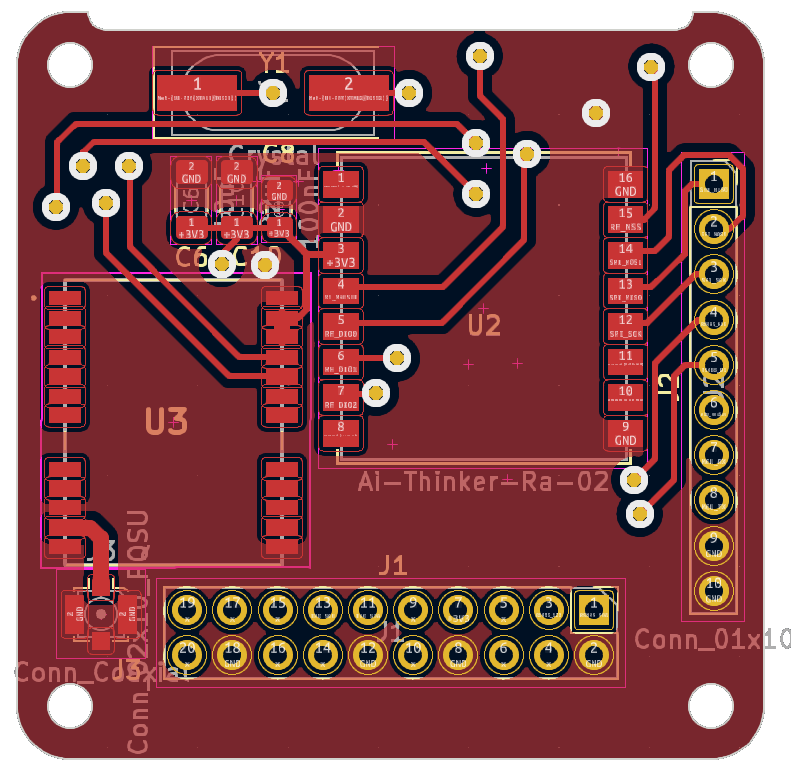
\includegraphics[width=.9\linewidth]{pqunit_pcb_design_front}
    \captionof{figure}{PocketQube Unit PCB Design (Front)}
    \label{fig:pqunit_pcb_design_front}
  \end{minipage}
  \begin{minipage}{.43\textwidth}
    \centering
    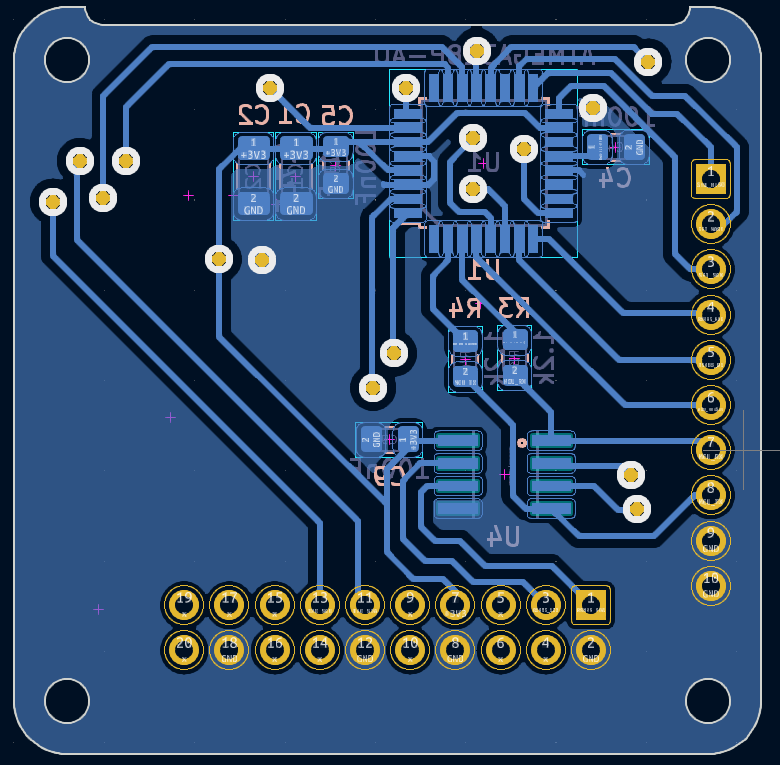
\includegraphics[width=.9\linewidth]{pqunit_pcb_design_back}
    \captionof{figure}{PocketQube Unit PCB Design (Back)}
    \label{fig:pqunit_pcb_design_back}
  \end{minipage}
  \end{figure}

The final PCB was designed to conform to the PocketQube standard, as shown in Figures \ref{fig:pqunit_pcb_design_front} and \ref{fig:pqunit_pcb_design_back}.